\section{Results}
\subsection{The Finite Difference Approach}
Eqn. \ref{ForceStressTemp} shows that the body force due to a temperature gradient can be inferred from the temperature variation of the stress--tensor. 
To first order, the temperature gradient of the stress--tensor can be calculated using a finite difference approach across a small temparature variation as
\begin{equation}
\label{FinDiff}
\left( \frac{\partial \sigma_{xx}(z,x)}{\partial T} \right) \approx \frac{\sigma_{xx}^{T_{2}}(z,x) - \sigma_{xx}^{T_{1}}(z,x)}{T_{2} - T_{1}}.
\end{equation}
Using this approximation it should, in principle, be possible to compute the Marangoni flow profile for an interface as follows:
\begin{enumerate}
	\item Compute $\sigma_{xx}(z)$ for an equilibrium system at a given temperature $T_{1}$.
	\item Repeat the calculation for another equilibrium system at slightly higher temperate $T_{2}$.
	\item Approximate the temperature gradient of the stress tensor using the finite difference approach (Eqn. \ref{FinDiff}).
	\item Infer $f_{x}(z)$ using Eqn. \ref{ForceStressTemp} to calculate a force profile.
	\item Compute the flow profile by applying $f_{x}(z)$ as an artifical body force to a non-equilibrium simulation at a suitable intermediate temperature $T_{3}$ (i.e. $T_{1} < T_{3} < T_{3}$).
\end{enumerate}

This method is used in the remainder of this chapter to investigate the Marangoni flow arising at a liquid--liquid interface. 

\subsection{Using a periodic binary-mixture}
The purest system to study is the case of a symmetrical binary--mixture under three-dimensional periodic boundary conditions, whereby the only deviation from a simple bulk fluid is the presence of two interfaces within the periodic unit box. 
In this case and forces arising within the fluid can only arise from the effects of the interfaces on the fluid.

This system can be generated using a Lennard--Jones fluid by controlling the relative interaction strengths of the two fluids (henceforth referred to as Fluid A and Fluid B).
To achieve a suitable level of miscibility of the fluids the values $\epsilon_{AA} = \epsilon_{BB} = 1.0$ and $\epsilon_{AB}=0.55$ were used, in agreement with the previous studies on symmetrical Lennard--Jones binary mixtures.\cite{MorenzoRazo,Blas}
The pressure was chosen to be $P=0.1$ and the temperature values used were $T=0.8$ and $T=0.9$, ensuring that for all simulations the system exists within the liquid region of the pLennard--Jones phase space.\cite{Smit}
With an absence of any bounding walls in the system, the fluid pressure and temperature were controlled using a Nos\'{e}--Hoover barostat and thermostat.

\begin{figure}[h]
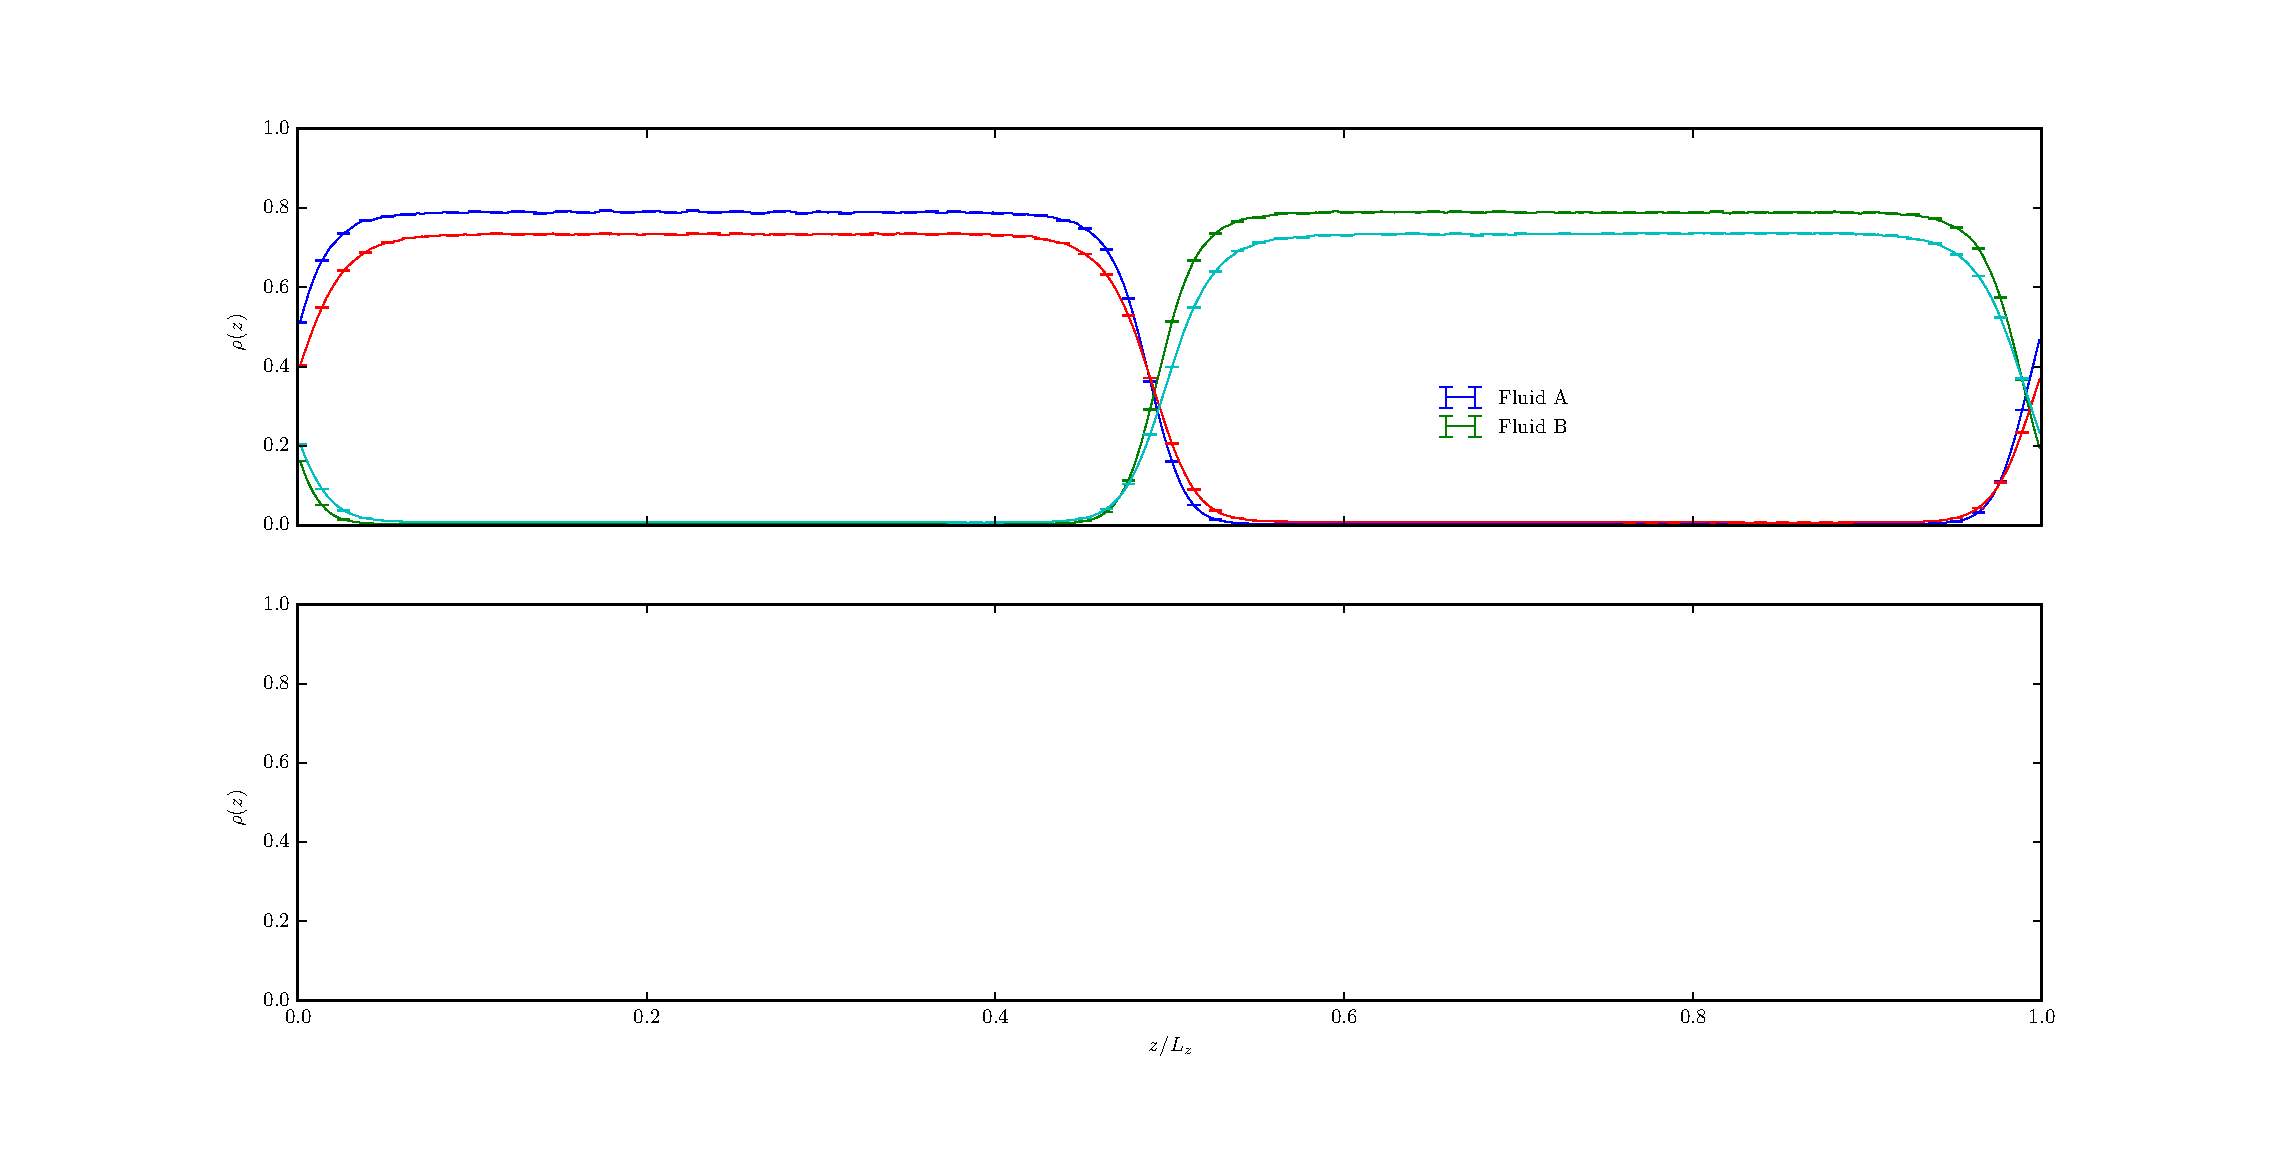
\includegraphics{AABBrho1mill}
\caption{The number density for the individual fluid components in a binary mixture simulated over $10^{6}$ timesteps clearly shows the immiscibility of the fluids. The interfacial region is relatively small and the number densities are uniform in the bulk regions, confirming the liquid state of the system.}
\label{AABBrho1mill}
\end{figure}
\subsection{Simulations over $10^{6}$ timesteps}

\begin{figure}[h]
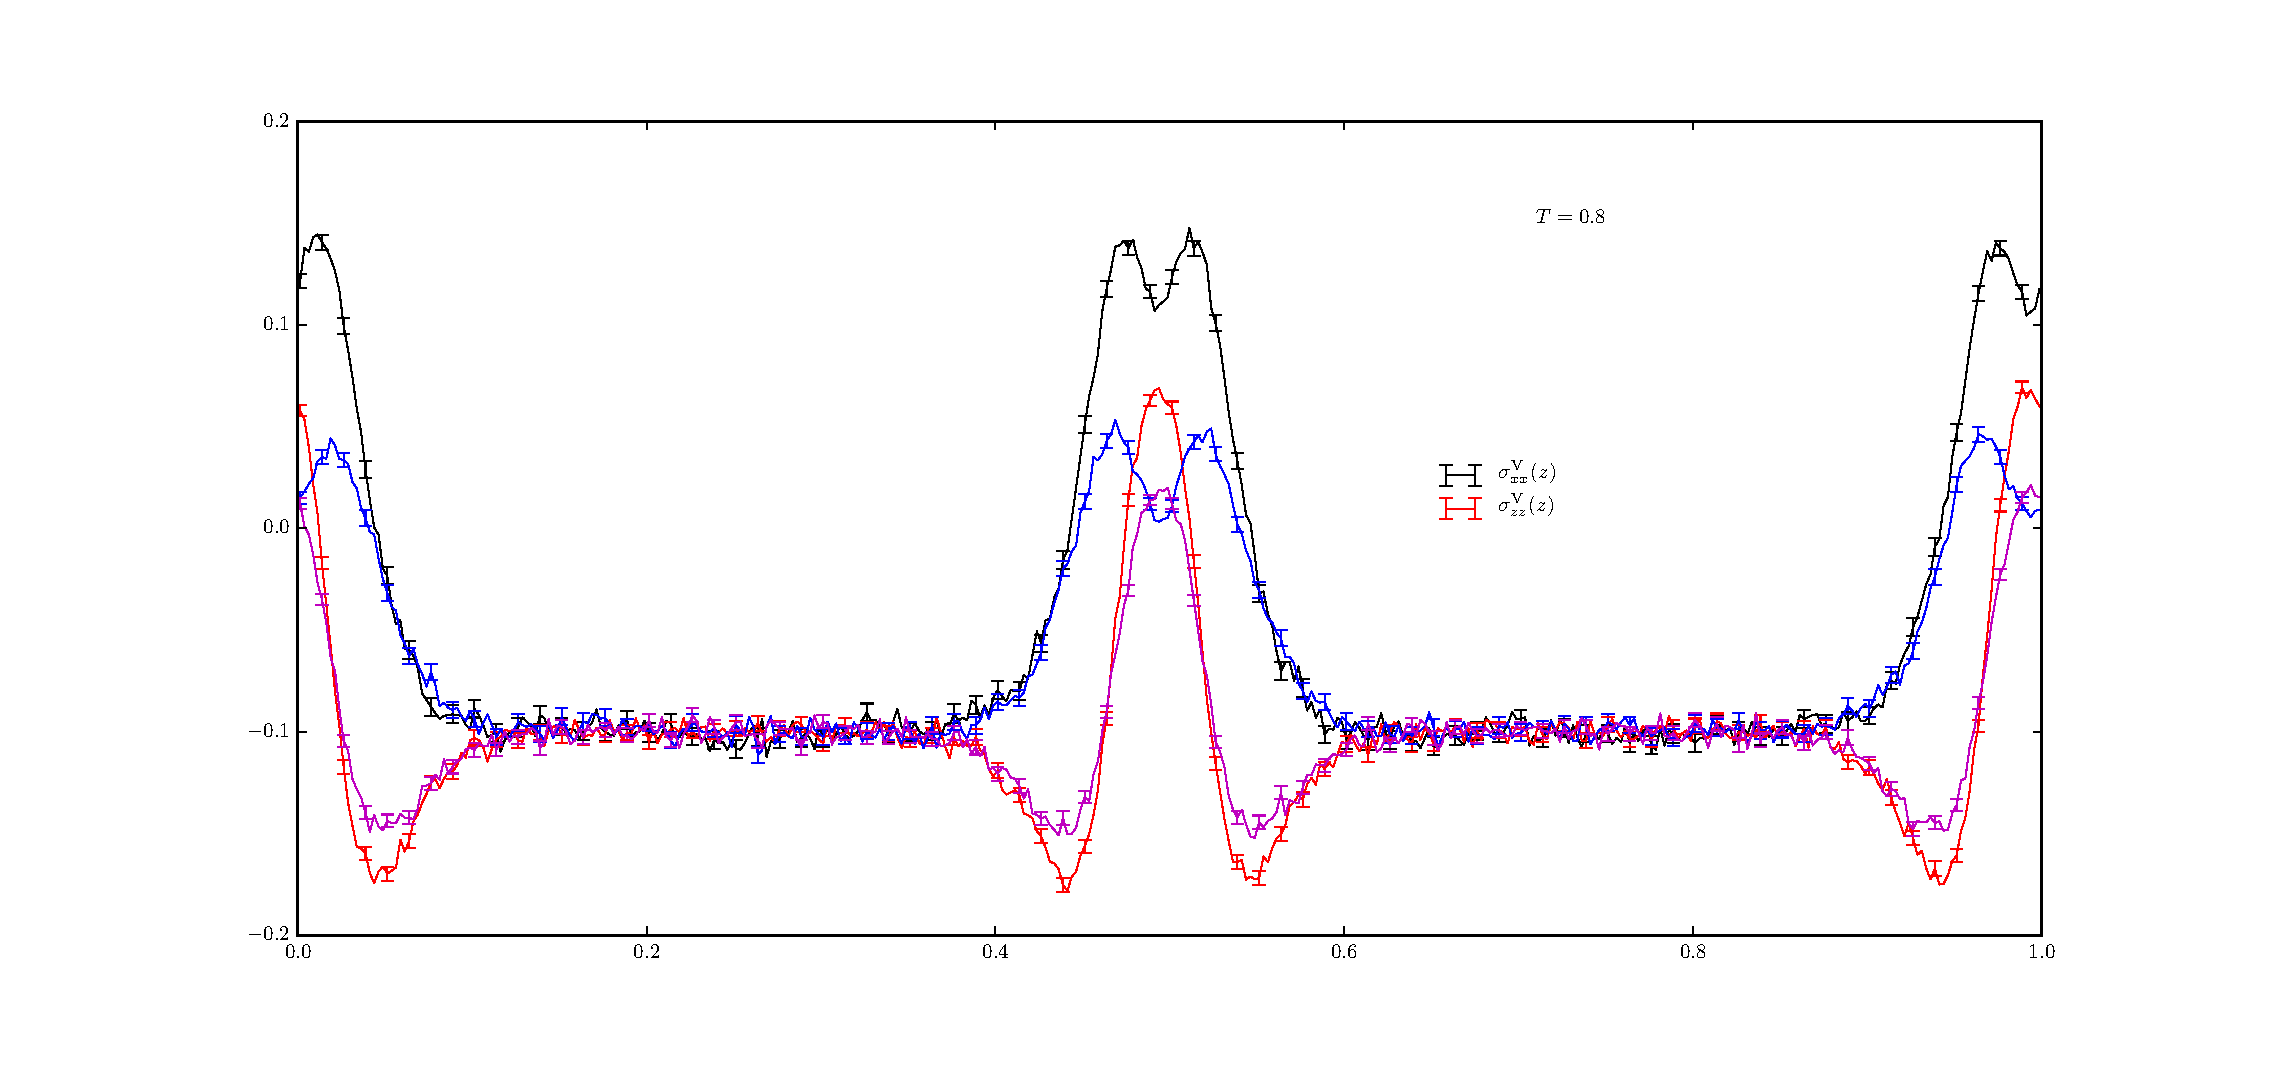
\includegraphics{AABBvir1mill}
\caption{The tangential and normal components of the Virial stress--tensor are plotted for the entire fluid at both temperaturs for an equilibrium simulation over $10^{6}$ timesteps.
It is clear that this is simulation time is insufficient as the noise level in the data is unacceptably high, although the noise does lie within the statistical error confirming there are no unexpected fluctuations in the bulk.}
\label{AABBvir1mill}
\end{figure}
Two systems at $T=0.8$ and $T=0.9$ were initiated as solid lattices that (since unstable under the pressure and temperature conditions) were allowed to melt over an equilibriation time of $2000 \tau$ and using a timestep of $\delta t = 0.001\tau$. 
These systems were then monitored over a period of $1,000,000$ timesteps and the average values of $\sigma^{\mathrm{IK}}(z)$, $\sigma^{\mathrm{V}}(z)$ and $\rho(z)$ were calculated.
Using these data, the density and stress profiles are plotted in Figures \ref{AABBrho1mill}, \ref{AABBvir1mill} and \ref{AABBik1mill}.

Whilst there does appear to be some form of Marangoni force occuring at the interface, it is clear that the level of noise in these data is too large to make any meaningful interpretation (although it is worth noting that the noise lies within the statistical error bars, of which only every 5 are shown for clarity). 
To reduce the amount of noise would require either a longer simulation run or a larger system size, both of which dramatically increase the computational cost of the simulation.
This is not particularly significant for calculating the virial stress since this can be computeddd within the LAMMPS package. 
However, the Irving--Kirkwood stress must be calculated through a post-processing method and is very expensive.

\FloatBarrier
\subsection{Simulations over $10^{7}$ timesteps}

\FloatBarrier
\subsection{Simulation over $3\times 10^{7}$ timesteps}
Whilst the Irving--Kirkwood is simply too expensive to run over such a long time period, it is possible to generate a more precise virial force profile by running the simulation over $3\times 10^{7}$ timesteps.
The tangential component of the fluid stress--tensor for each temperature is plotted in Figure \ref{AABBvir30mill} and shows significantly less noise than those shown in Figure \ref{AABBvir1mill} or Figure \ref{AABBvir10mill}.
\begin{figure}[h]
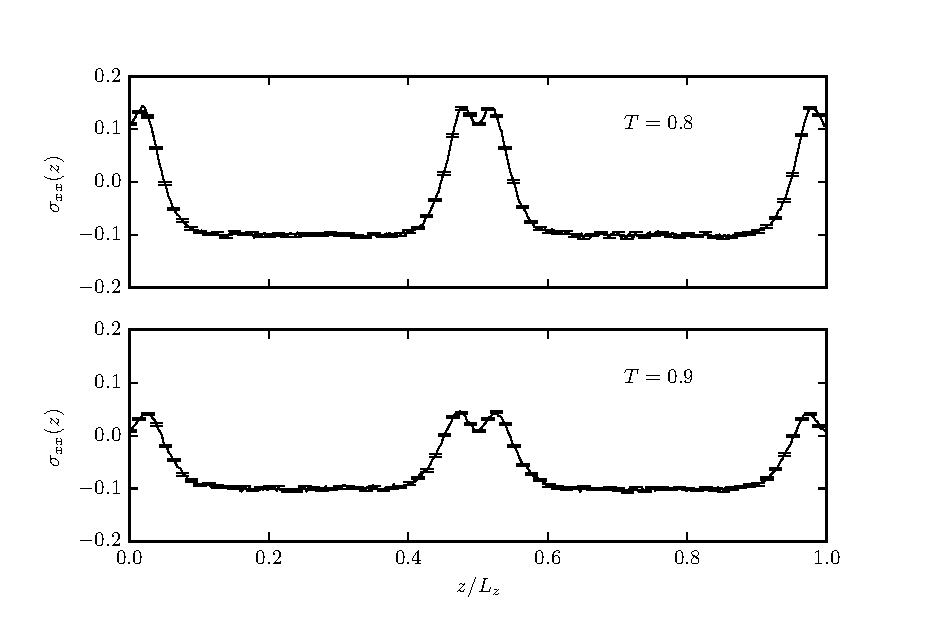
\includegraphics{AABBvir30mill}
\caption{Running the simulation over $3\times 10^{7}$ timesteps shows a dramatic reduction in the noise level in the tangential Virial stress--tensor components and in the statistical error.
However, there is also a slight (and unpredictable) deviation in the position of the interface.
After recentering, it is possible to use this data to infer the Marangoni body force with a manageable level of noise.}
\label{AABBvir30mill}
\end{figure}

\begin{figure}[h]
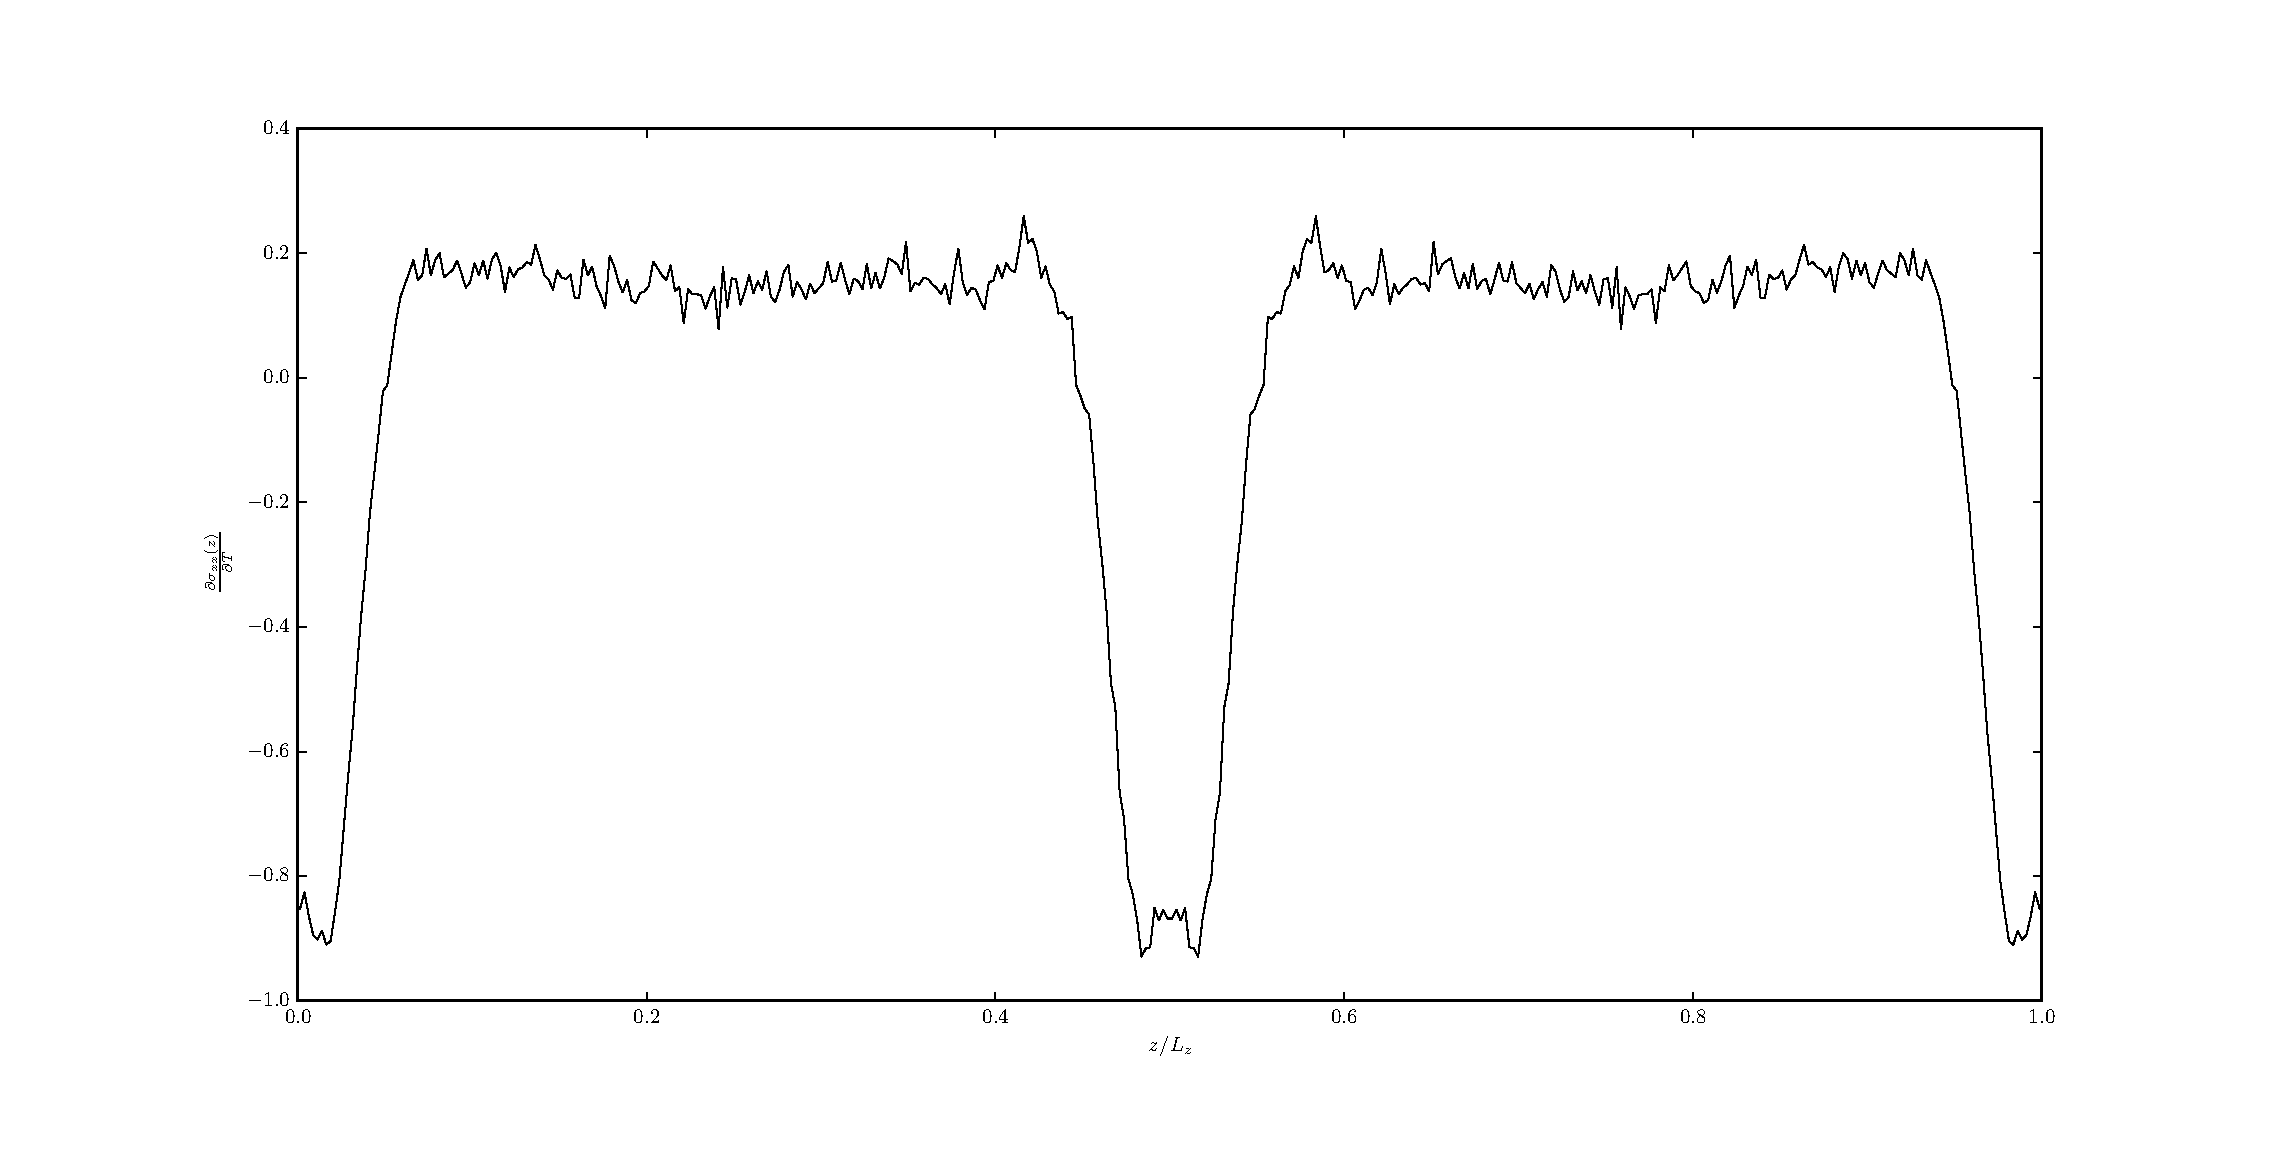
\includegraphics{AABBsymForce30mill}
\caption{The body forces for a binary--mixture infered from equilibrium simulations over $3\times 10^{7}$ timesteps is used to calculate a symmetric force profile which has no overall net force.
This profile shows a clear force at the interface representing the Marangoni force along with an opposing force for the bulk fluid implying the existence of a bulk back--flow (thus achieving no net flow).}
\label{AABBsymForce30mill}
\end{figure}

However upon closer inspection it is clear that the position of the interface has moved in the z-direction, although only by around $\frac{1}{400}^{th}$ of the box size. 
This irregularity is most likely to be an artefact from the divergence of molecular dynamics simulations over long time periods and can be removed by manually recentering the data to enfore the coincidence of the interface.
This may then be adjusted such that there is no net force on the fluid and then improved once more by noting that since the system is symmetric, so must be the force profile and thus by averaging between the force profile and its mirror image, a symmetrised force profile can be obtained as shown in Figure \ref{AABBsymForce30mill}.
